\documentclass[11pt]{beamer}
\usetheme{Antibes}
\usepackage[utf8]{inputenc}
\usepackage[german]{babel}
\usepackage[T1]{fontenc}
\usepackage{amsmath}
\usepackage{amsfonts}
\usepackage{amssymb}
\usepackage{graphicx}
\author{Gruppe C14 \\ Julián Häck,\textbf{ Martin Koytek}, Lars Wenning, Erik Zimmermann}
\title{Wärmelehre}
\usepackage{float}
\usepackage{subfigure}
\usepackage{multicol}
%\setbeamercovered{transparent} 
%\setbeamertemplate{navigation symbols}{} 
%\logo{} 
%\institute{} 
%\date{} 
%\subject{} 
\begin{document}
\setbeamertemplate{footline}[frame number]
\begin{frame}
\titlepage
\end{frame}

\section{Messung der Verdampfungsenthalpie}
\begin{frame}{Messung der Verdampfungsenthalpie}
\begin{equation*}
\frac{dp}{dT}=\frac{\nu \Lambda}{T(V_1-V_2)}
\end{equation*}
\begin{equation*}
\ln(p)=-\frac{\Lambda}{R}\cdot \frac{1}{T}+c \text{ mit } c=const
\end{equation*}
\end{frame}

\section{Rauschmessung}
\subsection{Temperatursensoren}
\begin{frame}{Rauschmessung}
\begin{figure}[H]
    \subfigure[Gruppe 1]{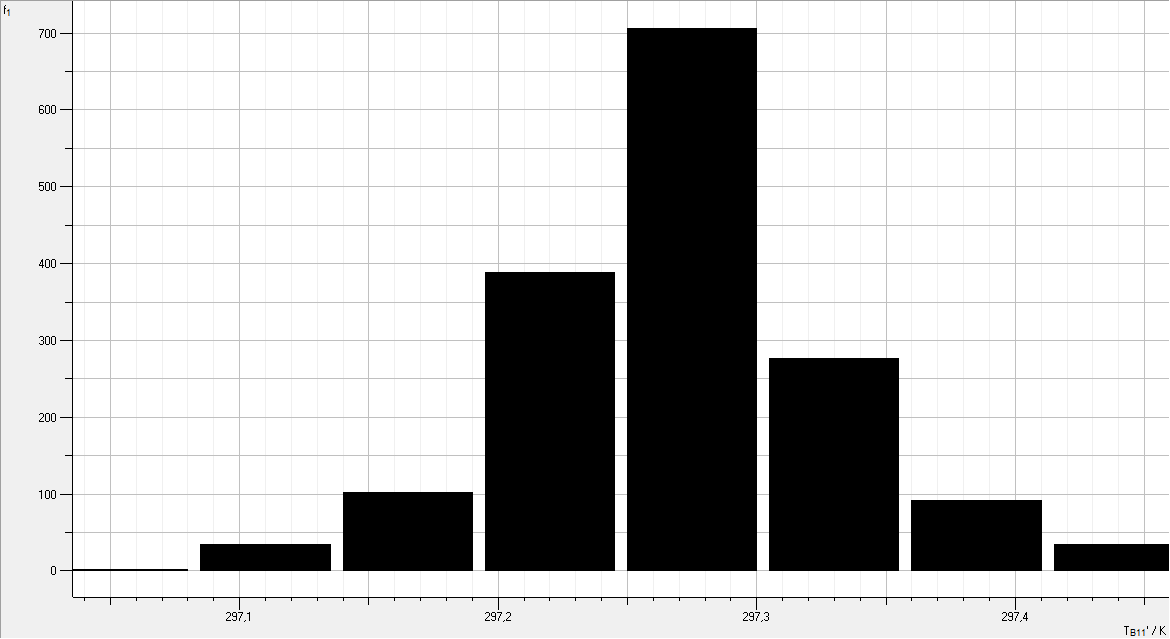
\includegraphics[width=0.49\textwidth]{Bilder/Zimmertemperatur_G1_1.png}}
    \subfigure[Gruppe 2]{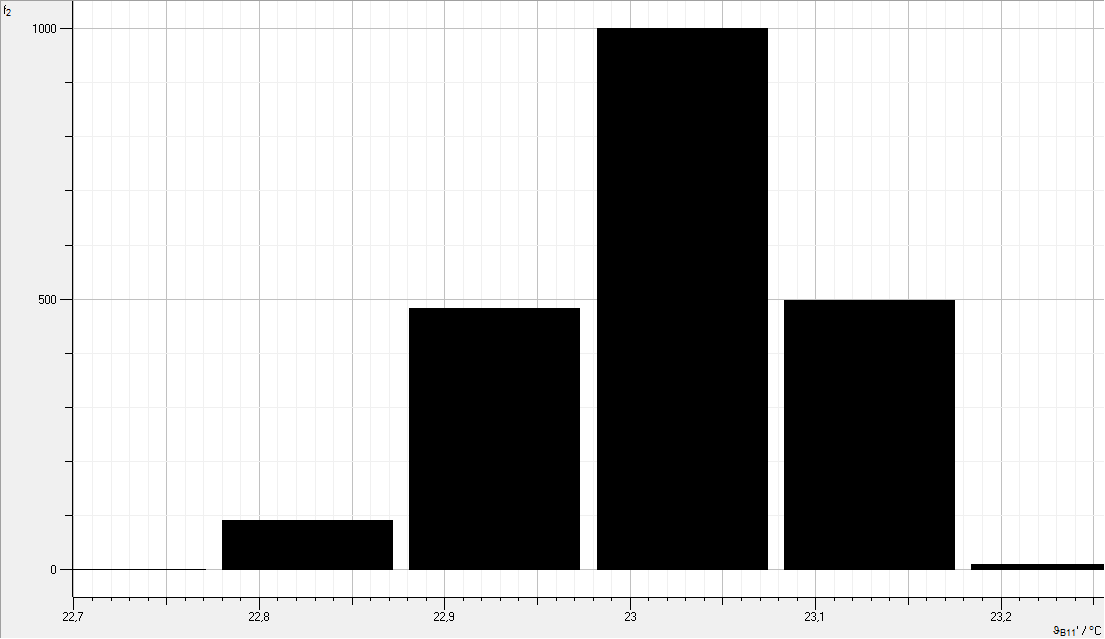
\includegraphics[width=0.49\textwidth]{Bilder/Zimmertemperatur_G2.png}}
\end{figure}
\begin{table}[H]\centering
\begin{tabular}{c|c|c}
 & Gruppe 1 & Gruppe 2 \\ 
\hline 
$T_M$ in K & 297.26 & 296.17 \\ 
$\sigma_T$ in K & 0.054 & 0.069 \\  
\end{tabular} 
\end{table}
\end{frame}



\subsection{Drucksensoren}
\begin{frame}
\begin{figure}[H]
    \subfigure[Gruppe 1]{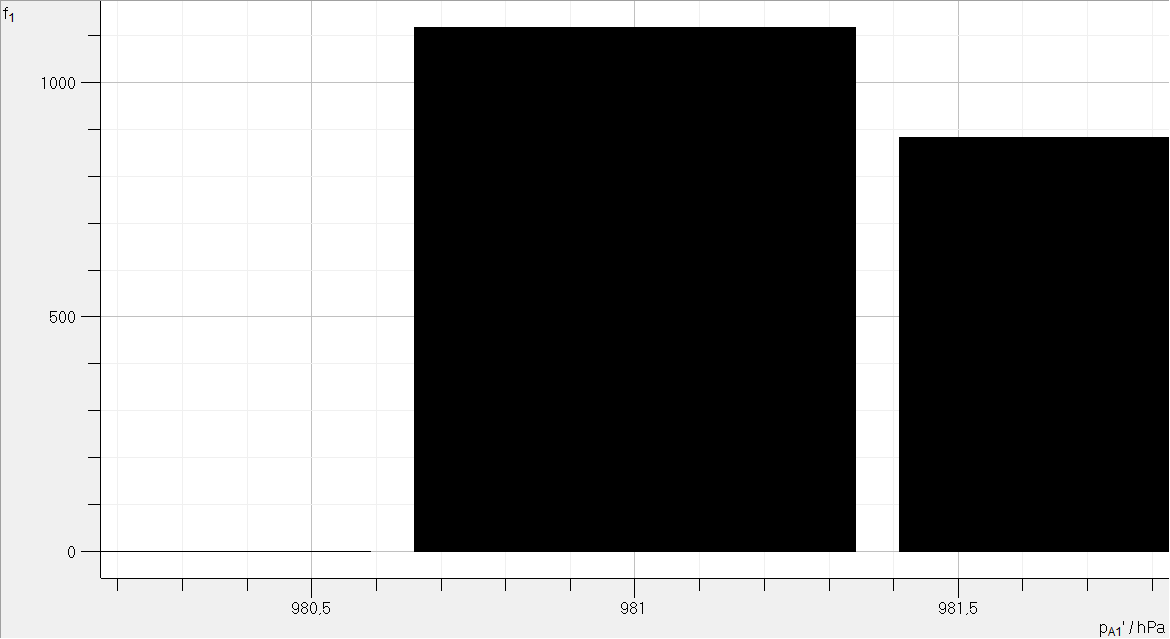
\includegraphics[width=0.49\textwidth]{Bilder/Zimmertemperatur_Druck_G1_1.png}}
    \subfigure[Gruppe 2]{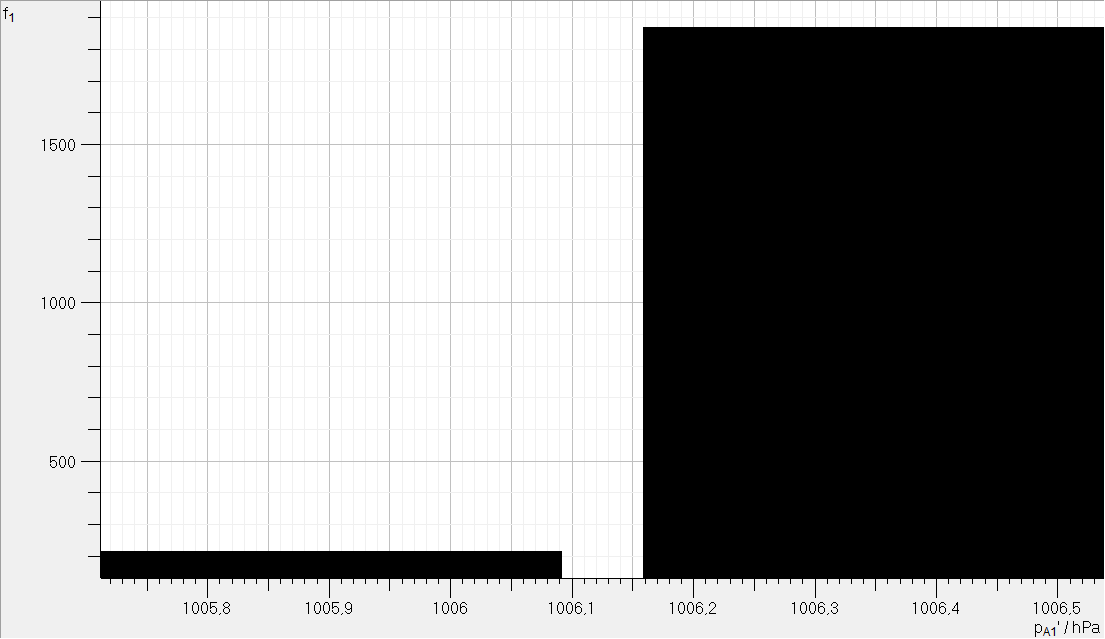
\includegraphics[width=0.49\textwidth]{Bilder/Zimmertemperatur_Druck_G2.png}}
\end{figure}

\begin{table}[H]\centering
\begin{tabular}{c|c|c}
 & Gruppe 1 & Gruppe 2 \\ 
\hline 
$P_M$ in hPa & 981.443 & 1006.265 \\ 
$\sigma_P$ in hPa & 0.370 & 0.348 \\  
\end{tabular} 
\end{table}
\end{frame}
\section{Temperaturkalibrierung}
\begin{frame}{Temperaturkalibrierung}
\begin{equation*}
T_{R}=aT_{C}+b
\end{equation*}
\begin{equation*}
T_{R}=a_1(T_{C}-\bar{T})+b_1
\end{equation*}
\begin{table}[H]\centering
\begin{tabular}{|c|c|}
\hline 
$T_R$ & $T_C$ \\ 
\hline 
273.16K & 274.277 \\ 
\hline
372.50 K & 372.227 \\ 
\hline
\end{tabular}
\end{table}

 
\end{frame}

\begin{frame}
\begin{figure}[H]
\centering
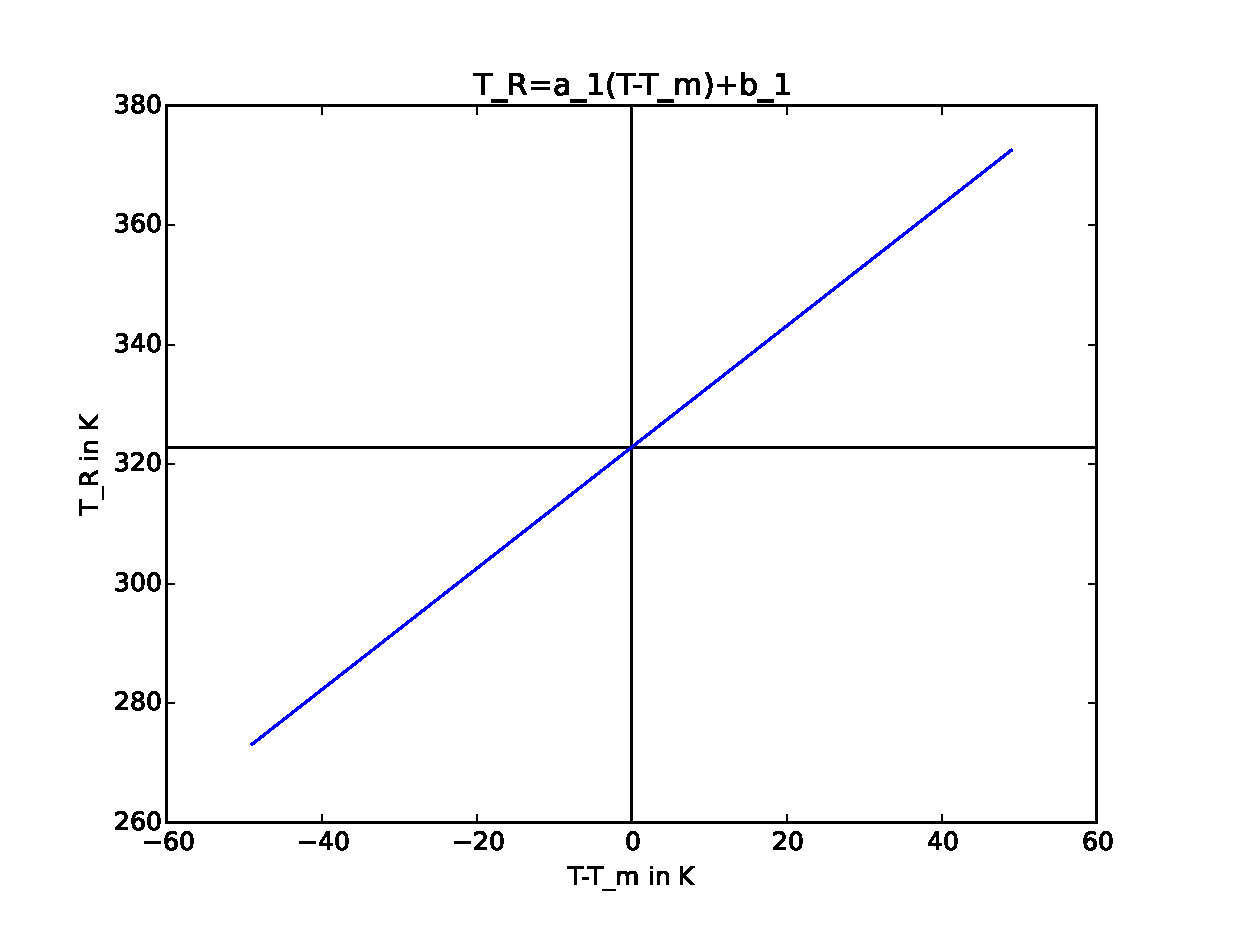
\includegraphics[scale=0.4]{Bilder/gewollteFunktion.eps}
\end{figure}
\begin{equation*}
a_1=1.015, \hspace{1cm} \sigma_{a_1}=2.955 \cdot 10^{-5}
\end{equation*}
\begin{equation*}
b_1=322.86 K, \hspace{1cm} \sigma_{b_1}=0.013 K
\end{equation*}
\end{frame}

\begin{frame}
\begin{equation*}
\sigma_{T_{R}} = \sqrt{((T_C-\bar{T}) \sigma_a)^2+\sigma_b^2}=0.0137
\end{equation*}

\begin{equation*}
\sigma_{\lambda_{T}}=\frac{\sigma_T}{T}\cdot \Lambda \approx 0.002 \frac{kJ}{mol}
\end{equation*}
\begin{table}[H]\centering
\caption{Systematische Fehler aus Herstellerangaben: Druck}
\begin{tabular}{|c|c|}
\hline 
Linearitätsfehler & $\pm 1\%$ \\ 
\hline 
Sensor & $\pm 1\%$ \\ 
\hline 
Verstärkungsfehler & $\pm 1\%$ \\ 
\hline 
\end{tabular}
\end{table}


\begin{table}[H]\centering
\caption{Systematische Fehler aus Herstellerangaben: Temperatur}
\begin{tabular}{|c|c|}
\hline 
Sensor & $\pm 2.5 K $ \\ 
\hline 
Konverter & $\pm 1\%$ \\ 
\hline 
\end{tabular}
\end{table}
\end{frame}

\section{Druckkalibrierung}
\begin{frame}{Druckkalibrierung}
\begin{table}[H]\centering
\begin{tabular}{|c|c|c|c|}
\hline 
 & $p_{Cassy}$ & $p_{Wetterstation}$ & $\Delta p$ \\ 
\hline 
Gruppe 1 & 981.54 hPa & 985 hPa & 3.46 hPa \\ 
\hline 
Gruppe 2 & 1006.5 hPa & 984 hPa & 22.5 hPa \\ 
\hline 
\end{tabular} 
\end{table}
kein Beitrag zur Steigung.
\end{frame}

\section{Dichtigkeitsmessung}

\subsection{Aufbau}
\begin{frame}{Dichtigkeitsmessung}
\begin{figure}[H]
\centering
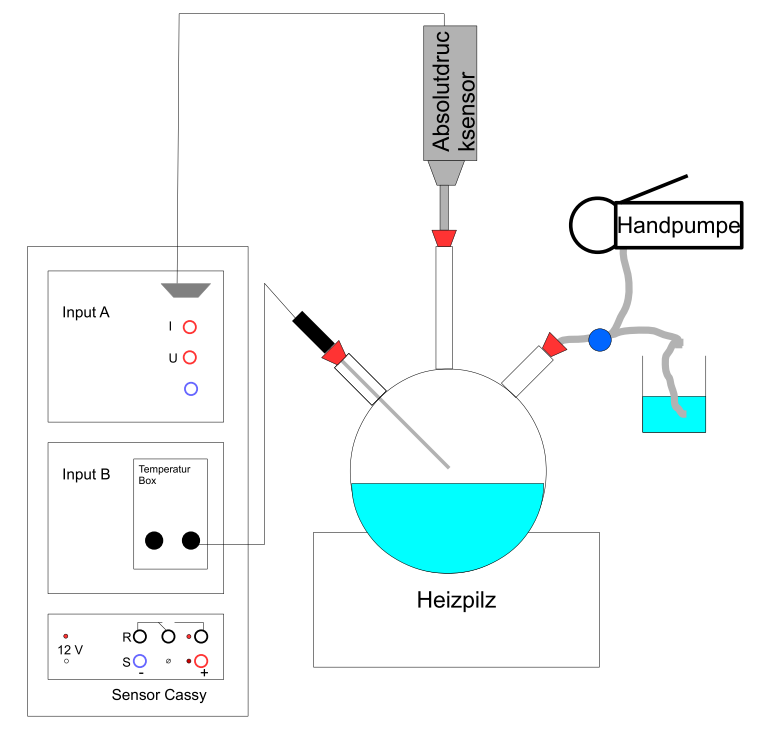
\includegraphics[scale=0.4]{Bilder/Versuchsskizze.PNG}
\end{figure}

\end{frame}

\subsection{Rohdaten}
\begin{frame}
\begin{figure}[H]
\centering
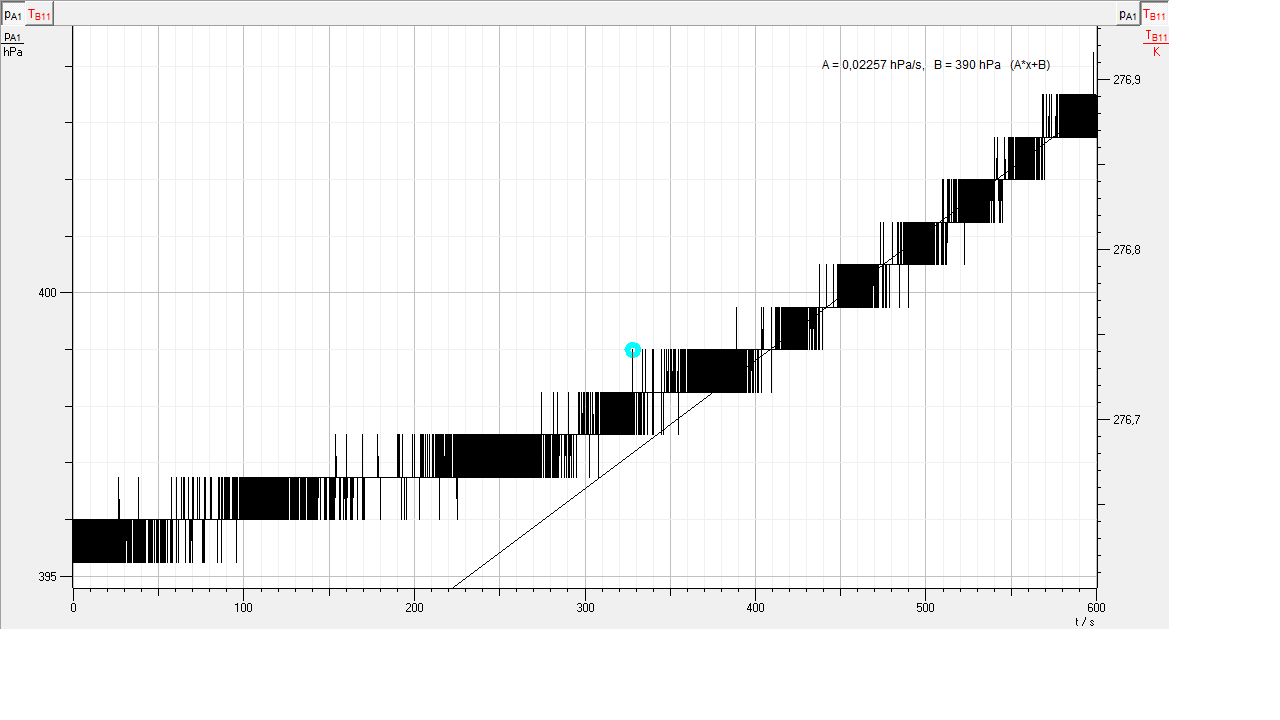
\includegraphics[scale=0.3]{Bilder/dichtigkeit_raw_JM.png}
\caption{Leckmessung Gruppe 1}
\end{figure}
\end{frame}

\begin{frame}
\begin{figure}[H]
\centering
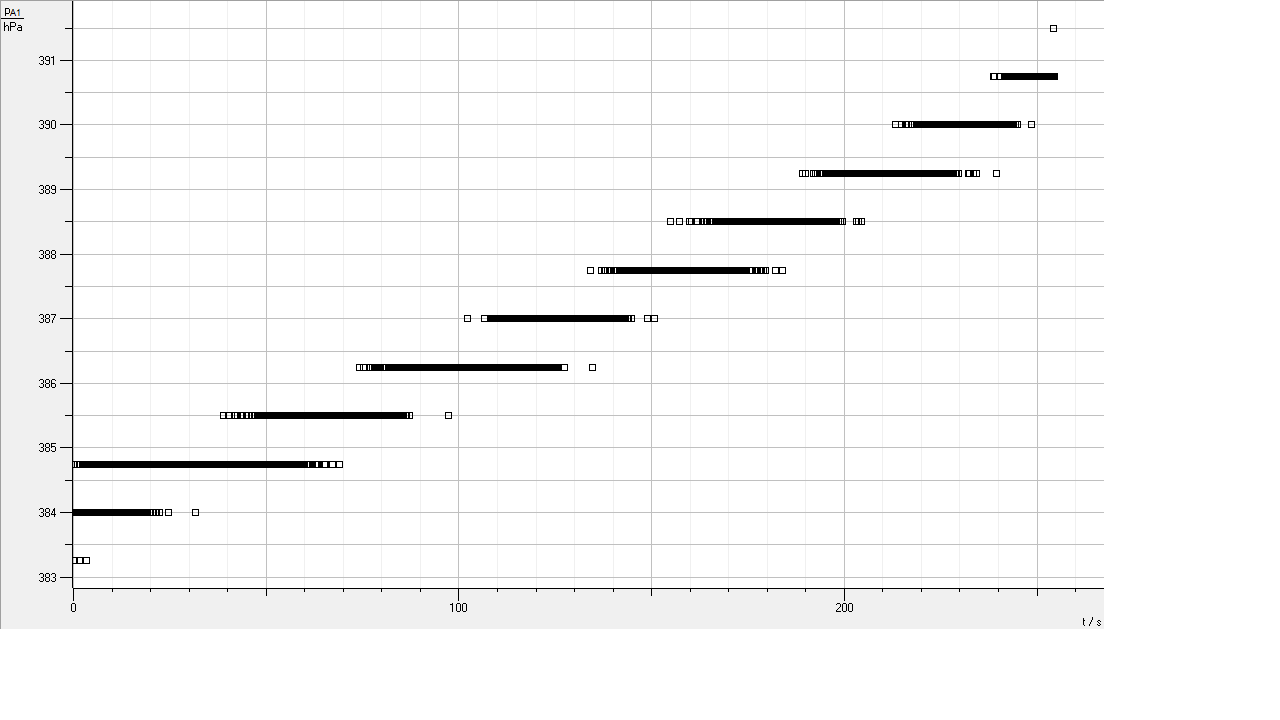
\includegraphics[scale=0.3]{Bilder/dichtigkeit_raw_EL.png}
\caption{Leckmessung Gruppe 2}
\end{figure}
\end{frame}

\subsection{Transformation der Rohdaten}
\begin{frame}
\begin{figure}[H]
\centering
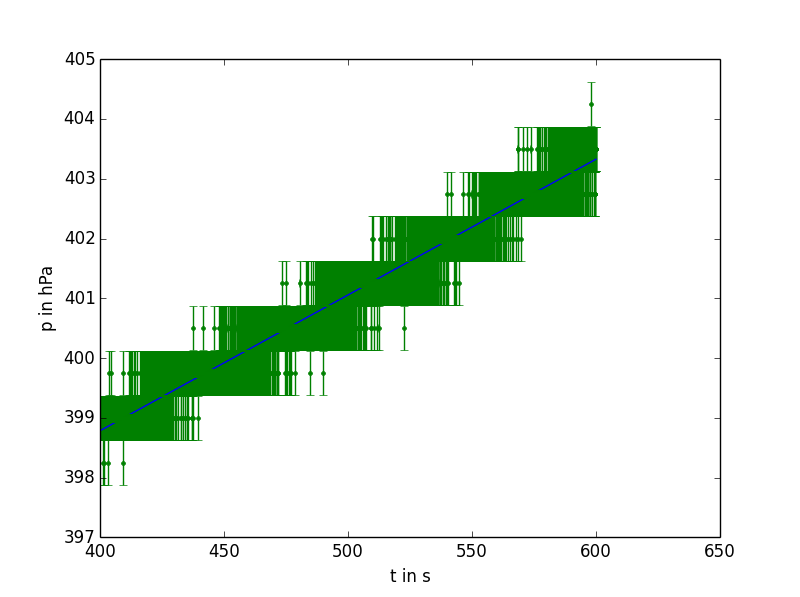
\includegraphics[scale=0.5]{Bilder/dichtigkeit__JM.png}
\caption{Lineare Regression Gruppe 1 $\frac{\chi^2}{f}=0.638$}
\end{figure}
Die Leckrate für Gruppe 1 beträgt 1.364$\,\frac{hPa}{min}$.
\end{frame}

\begin{frame}
\begin{figure}[H]
\centering
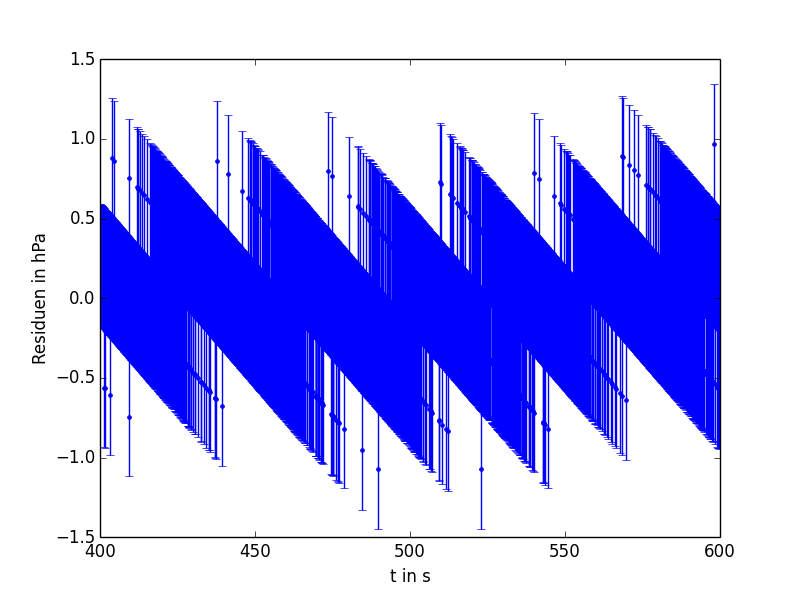
\includegraphics[scale=0.5]{Bilder/residuen_dichtigkeit_JM.png}
\caption{Residuen für die Anpassung von Gruppe 1}
\end{figure}
\end{frame}

\begin{frame}
\begin{figure}[H]
\centering
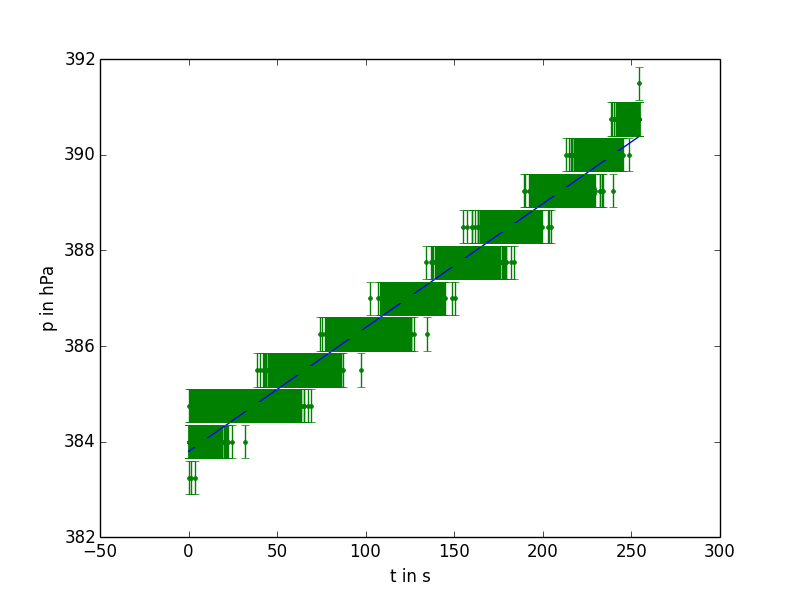
\includegraphics[scale=0.5]{Bilder/dichtigkeit__EL.png}
\caption{Lineare Regression Gruppe 2, $\frac{\chi^2}{f}=0.804$}
\end{figure}
Die Leckrate für Gruppe 2 beträgt 1.554$\,\frac{hPa}{min}$.
\end{frame}

\begin{frame}
\begin{figure}[H]
\centering
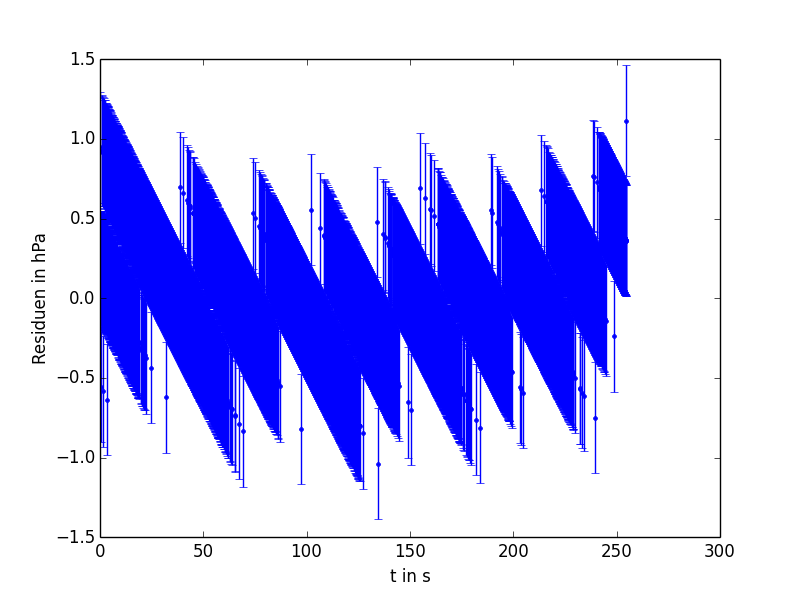
\includegraphics[scale=0.5]{Bilder/residuen_dichtigkeit_EL.png}
\caption{Residuen der Anpassung Gruppe 2}
\end{figure}
\end{frame}

\section{Messung der Verdampfungsenthalpie von Wasser}
\begin{frame}{Messung der Verdampfungsenthalpie}
\begin{equation*}
\frac{dp}{dT}=\frac{\nu \Lambda}{T(V_1-V_2)}
\end{equation*}
\begin{equation*}
\ln(p)=-\frac{\Lambda}{R}\cdot \frac{1}{T}+c \text{ mit } c=const
\end{equation*}
\end{frame}


\begin{frame}
\begin{figure}[H]
\centering
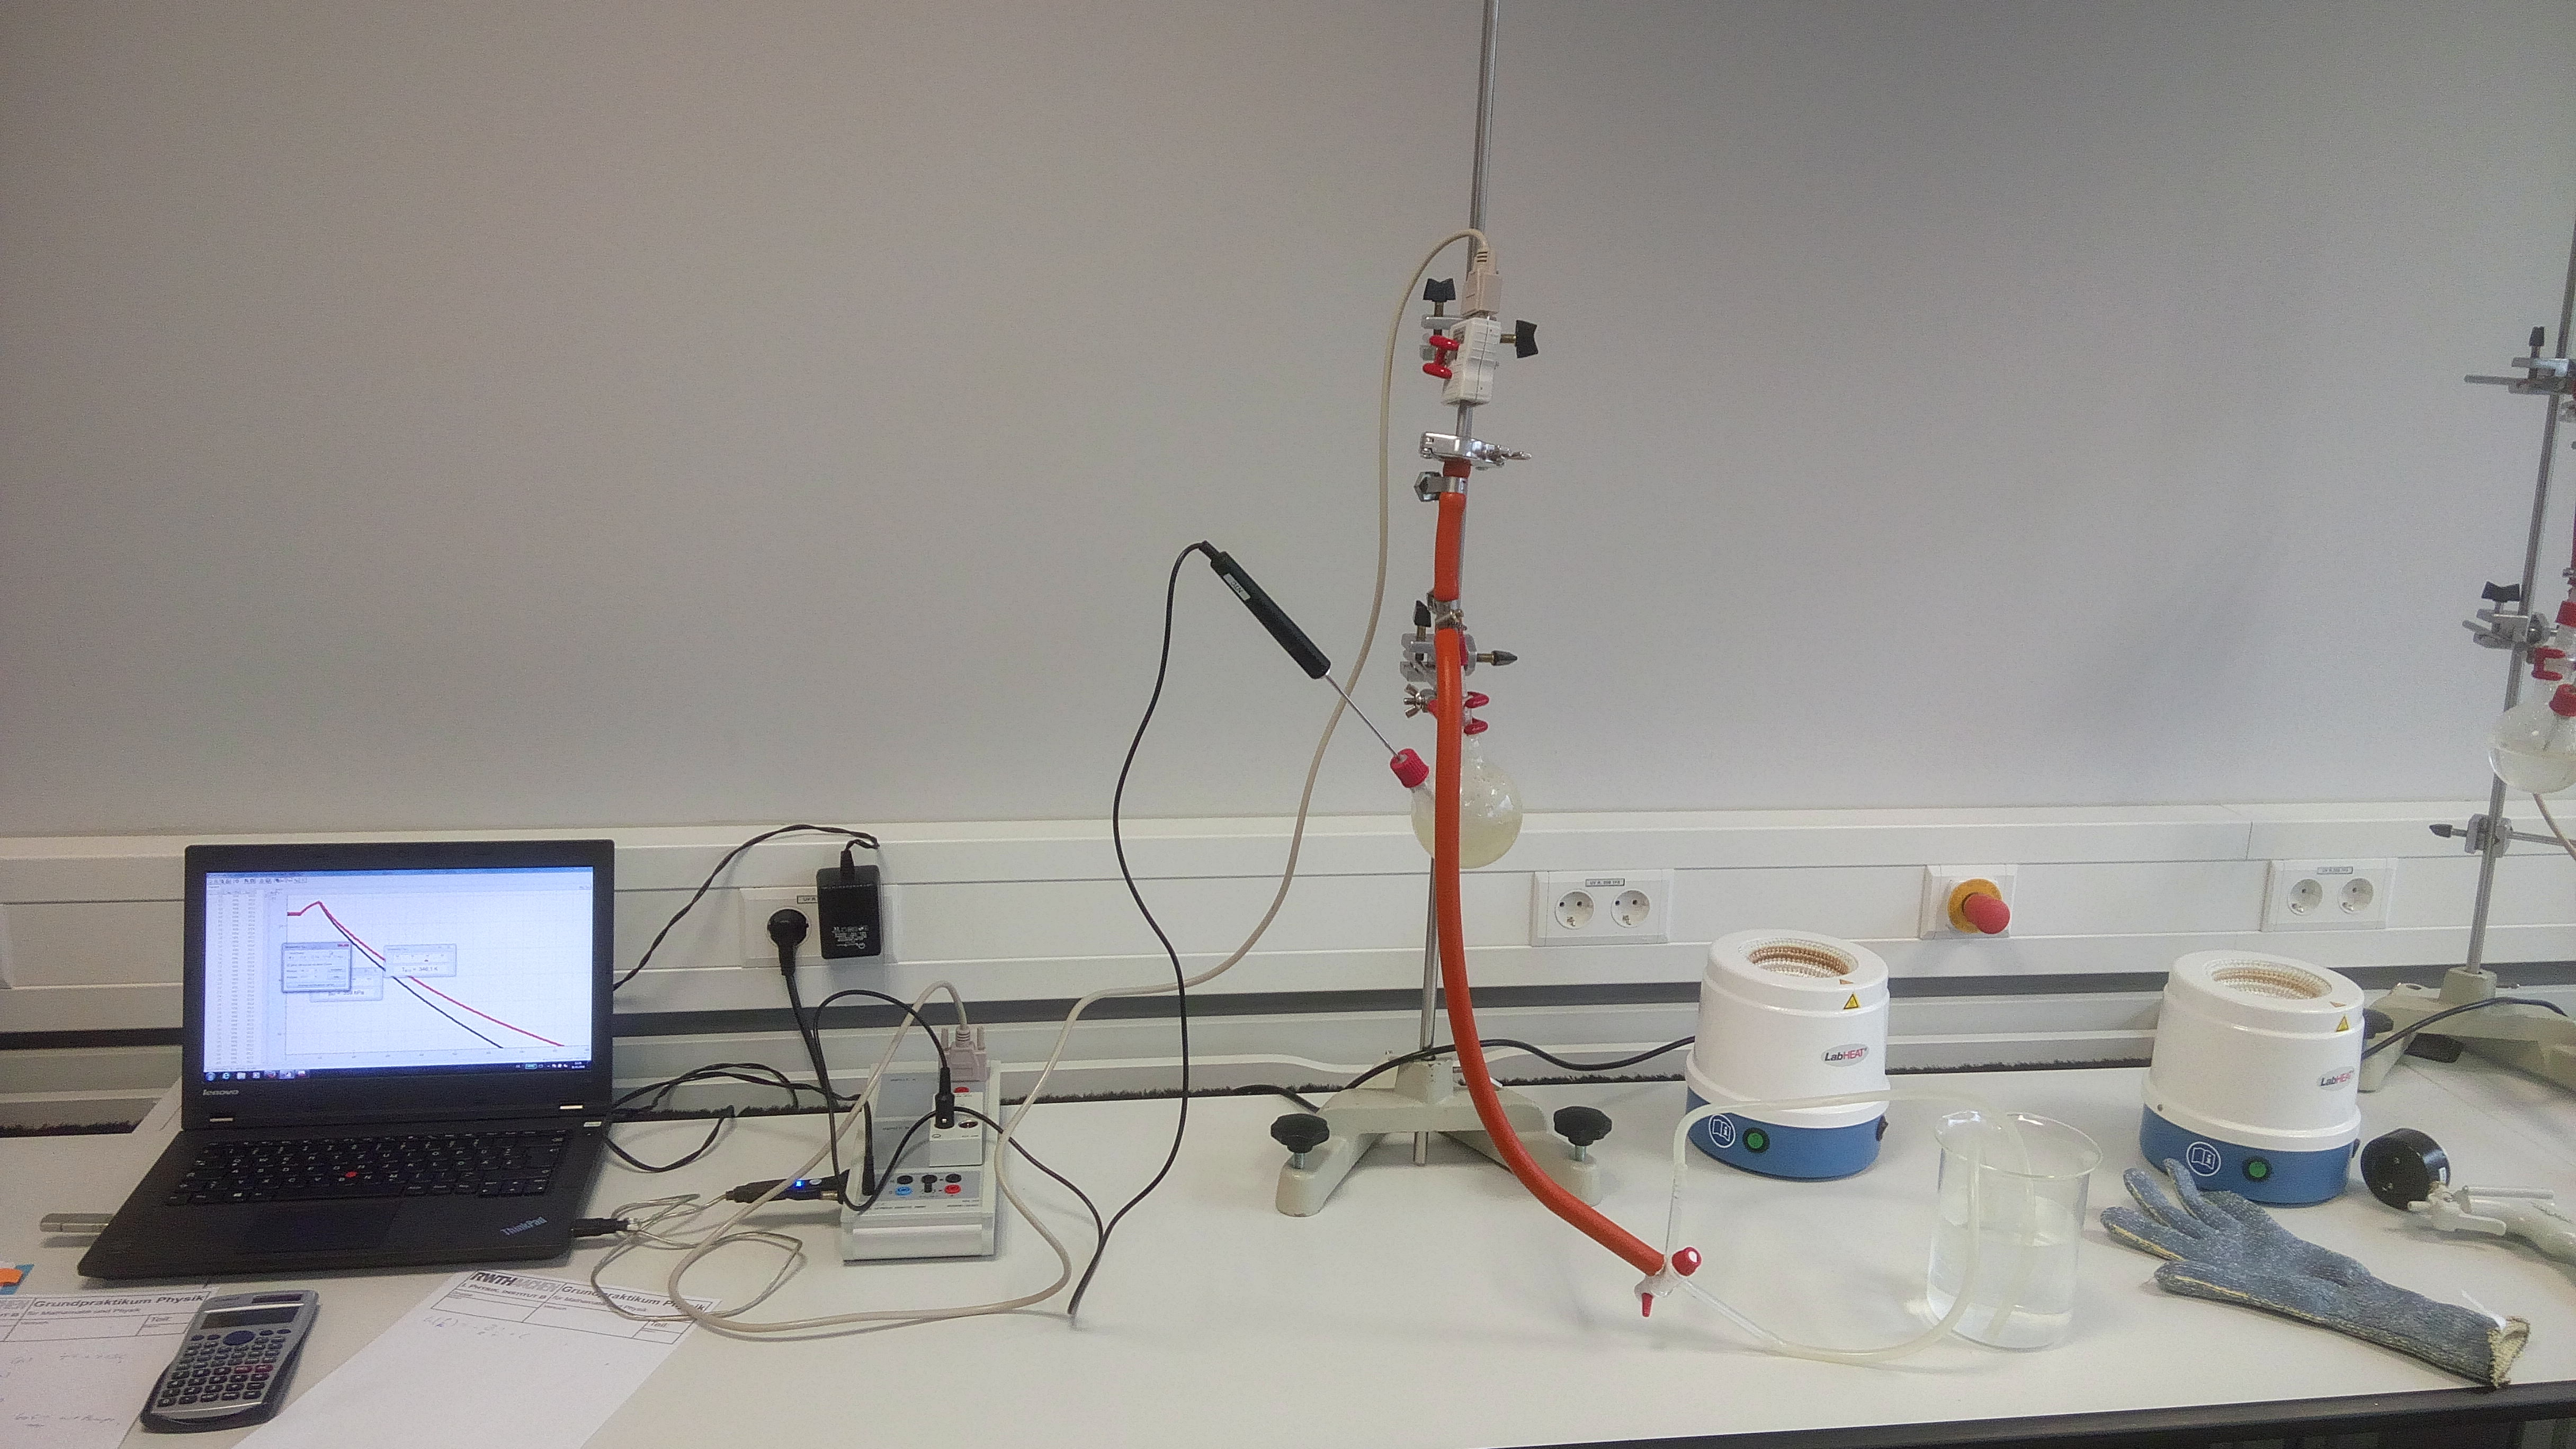
\includegraphics[scale=0.065]{Bilder/IMG_20160331_121650.jpg}
\end{figure}
\end{frame}

\subsection{Rohdaten}
\begin{frame}
\begin{figure}[H]
\centering
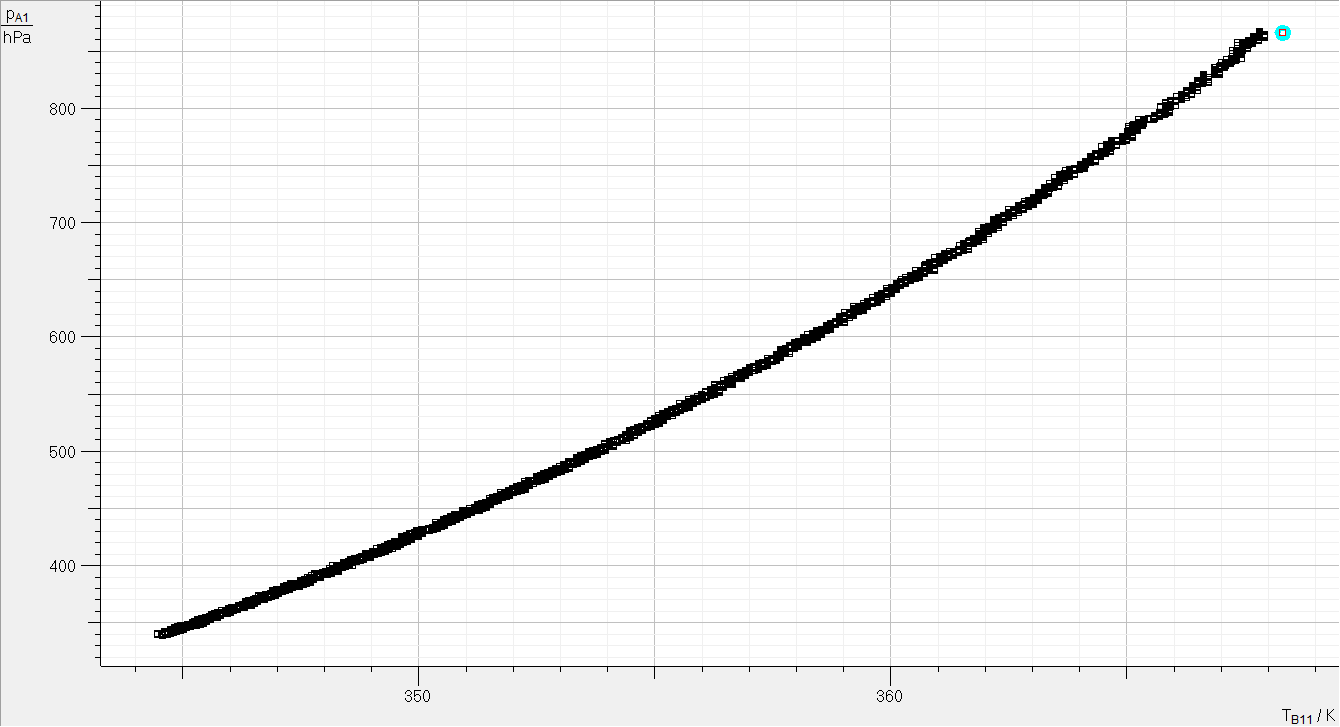
\includegraphics[scale=0.4]{Bilder/RohdatenHaupmessungGrp11.png}
\end{figure}
\end{frame}

\begin{frame}
\begin{figure}[H]
\centering
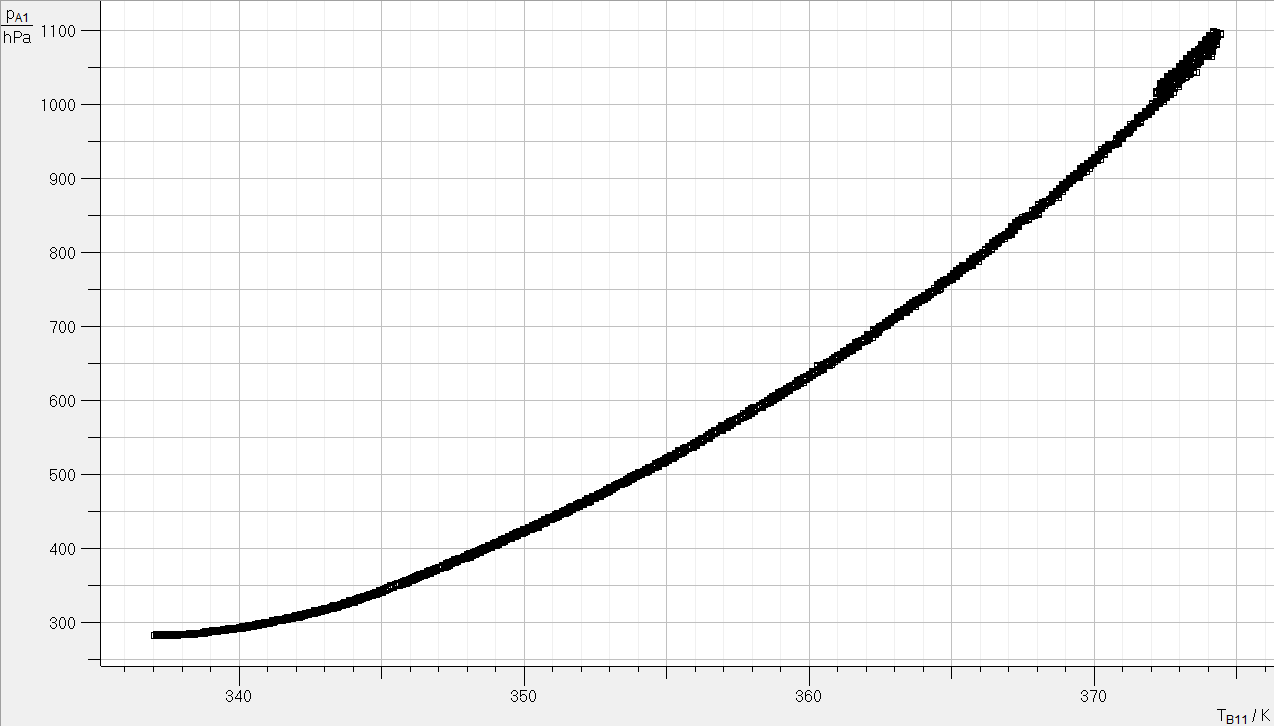
\includegraphics[scale=0.4]{Bilder/RohdatenHaupmessungGrp2.png}
\end{figure}
\end{frame}

\subsection{Transformation der Rohdaten}
\begin{frame}
\begin{figure}[H]
\centering
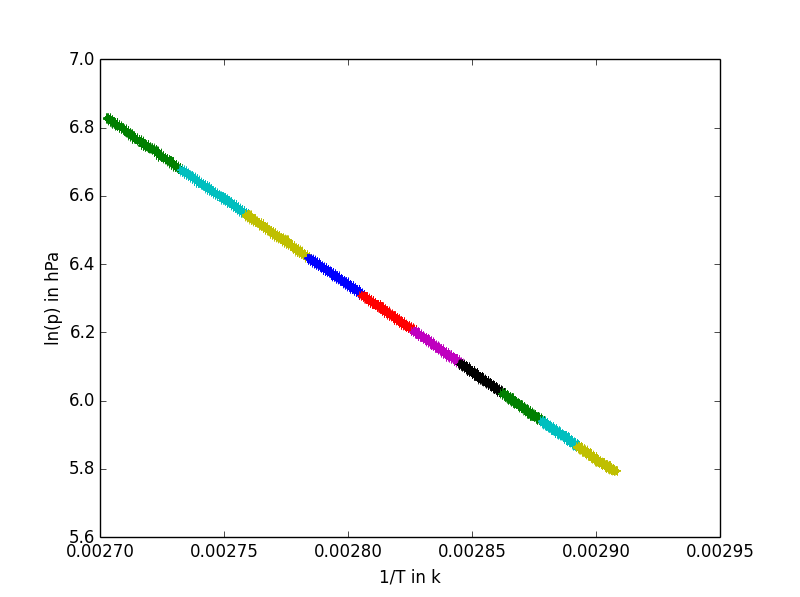
\includegraphics[scale=0.5]{Bilder/linreg_EL_neuerFehler.png}
\end{figure}
\end{frame}

\begin{frame}
\begin{figure}[H]
\centering
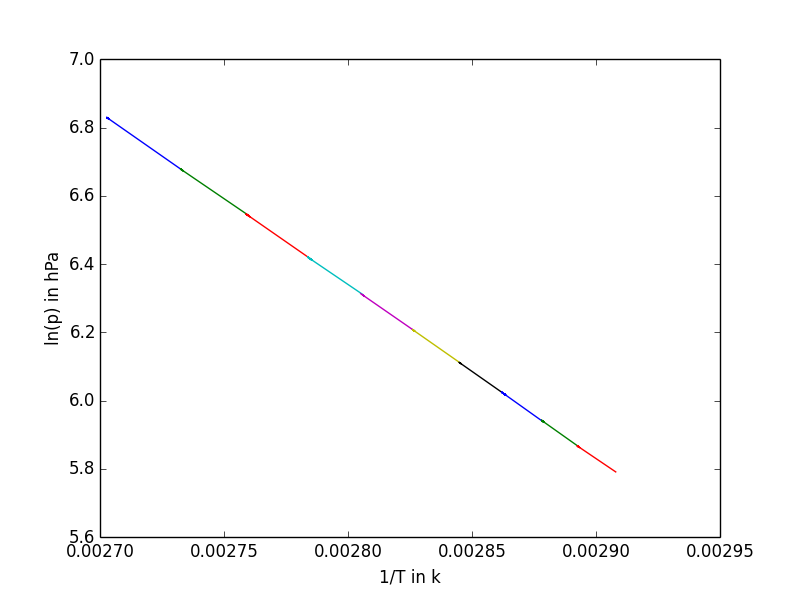
\includegraphics[scale=0.5]{Bilder/linreg_nurlinreg_EL.png}
\end{figure}
\begin{itemize}
\item $\frac{\chi^2}{f} \Rightarrow 1.27 | 0.96 | 1.12 | 0.86 | 0.89 | 0.77 | 0.79 | 0.78 | 0.71 | 0.74$
\end{itemize}
\end{frame}

\subsection{Ergebnisse}
\begin{frame}
\begin{equation*}
\ln(p)=-\frac{\Lambda}{R}\cdot \frac{1}{T}+c \text{ mit } c=const
\end{equation*}
\begin{table}[H]\centering
\begin{tabular}{c|c|c|c|c}
Abschnitt&T in K&$\Lambda$ in $\frac{kJ}{mol}$&$\sigma_{\Lambda_{stat}}$in $\frac{kJ}{mol}$&$\sigma_{\Lambda_{sys}}$in $\frac{kJ}{mol}$\\
\hline
1&367.93&42.18&0.273&0.518\\
2&364.13&41.17&0.156&0.508\\
3&360.76&41.96&0.102&0.518\\
4&357.71&40.97&0.1&0.508\\
5&355.03&41.8&0.12&0.519\\
6&352.6&42.24&0.117&0.525\\
7&350.38&42.31&0.136&0.527\\
8&348.4&43.03&0.141&0.537\\
9&346.54&42.79&0.162&0.535\\
10&344.83&40.84&0.175&0.512\\
\end{tabular}
\end{table}
zum Vergleich - $\Lambda_{Lit}=40.6\,\frac{kJ}{mol}$
\end{frame}

\subsection{Verdampfungswärme gg Temperatur}
\begin{frame}
\begin{figure}[H]
\centering
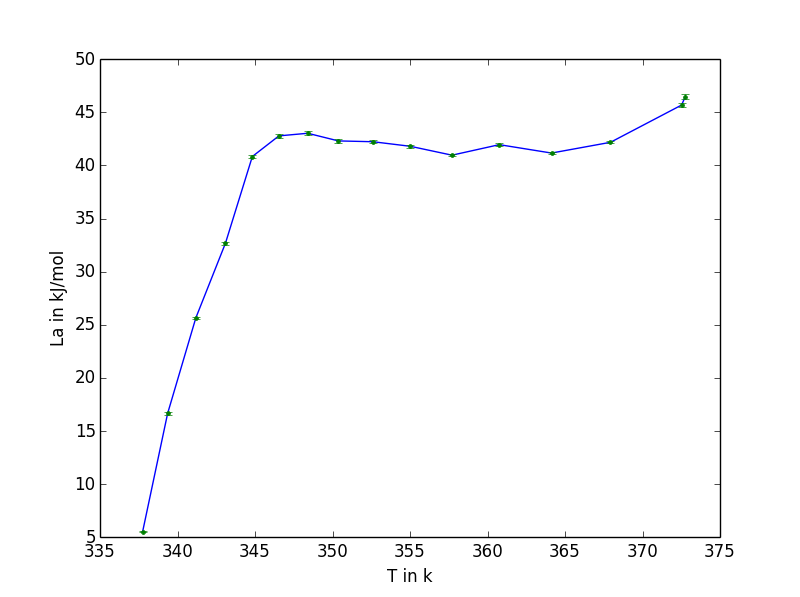
\includegraphics[scale=0.5]{Bilder/lamda_EL_neuerFehler.png}
\end{figure}
\end{frame}

\subsection{Fazit}
\begin{frame}
\begin{itemize}
\item Werte für $\Lambda$ zwischen 1 und 10 $\sigma$ um Literaturwert
\item fallende Verdampfungsenthalpie bei steigender Temperatur konnte verifiziert werden
\end{itemize}
\end{frame}


\end{document}